% !TeX program = xelatex
% Compile in this directory: latexmk -xelatex pyfracpaq-user-manual.tex
\documentclass[11pt,a4paper,oneside,parskip=half]{scrartcl}
\newcommand{\ManualTitle}{Manual do usuário}
\newcommand{\ManualDate}{Novembro de 2026}
\newcommand{\ManualAuthor}{Documentação do PyFracPaQ}
\newcommand{\ManualSubject}{Uso, teoria e exemplos SD11A}
\usepackage[brazilian]{babel}
% Shared layout and typography for both language editions.
\usepackage[margin=23mm,headheight=16pt,footskip=12mm]{geometry}
\usepackage{fontspec}
\setmainfont{texgyrepagella}[Extension=.otf,UprightFont=*-regular,BoldFont=*-bold,ItalicFont=*-italic,BoldItalicFont=*-bolditalic]
\setsansfont{texgyreheros}[Extension=.otf,UprightFont=*-regular,BoldFont=*-bold,ItalicFont=*-italic,BoldItalicFont=*-bolditalic]
\setmonofont[Scale=.86]{lmmono10-regular.otf}
\usepackage{unicode-math}
\setmathfont{texgyrepagella-math.otf}
\usepackage{graphicx,booktabs,tabularx,longtable,array}
\usepackage[dvipsnames]{xcolor}
\usepackage{enumitem,microtype,needspace,placeins,fancyhdr,lastpage,xurl}
\usepackage[most]{tcolorbox}
\definecolor{brand}{HTML}{126870}
\definecolor{ink}{HTML}{18323A}
\definecolor{pale}{HTML}{F0F6F6}
\usepackage[colorlinks=true,linkcolor=brand,urlcolor=brand,citecolor=brand,bookmarksnumbered=true,pdfencoding=auto]{hyperref}
\hypersetup{pdftitle={PyFracPaQ 0.9.0rc1 - \ManualTitle},pdfauthor={\ManualAuthor},pdfsubject={\ManualSubject}}
\graphicspath{{assets/}}
\setlength{\emergencystretch}{3em}
\setcounter{tocdepth}{2}
\setlist{nosep,topsep=5pt,leftmargin=*}
\setkomafont{section}{\sffamily\bfseries\color{brand}\Large}
\setkomafont{subsection}{\sffamily\bfseries\color{ink}\large}
\setkomafont{subsubsection}{\sffamily\bfseries\normalsize}
\pagestyle{fancy}\fancyhf{}
\fancyhead[L]{\small\sffamily PyFracPaQ / \ManualTitle}
\fancyhead[R]{\small\sffamily 0.9.0rc1}
\fancyfoot[L]{\footnotesize \ManualDate}
\fancyfoot[R]{\footnotesize\thepage\ / \pageref*{LastPage}}
\renewcommand{\headrulewidth}{.3pt}
\fancypagestyle{plain}{\fancyhf{}\fancyhead[L]{\small\sffamily PyFracPaQ / \ManualTitle}\fancyhead[R]{\small\sffamily 0.9.0rc1}\fancyfoot[L]{\footnotesize \ManualDate}\fancyfoot[R]{\footnotesize\thepage\ / \pageref*{LastPage}}\renewcommand{\headrulewidth}{.3pt}}
\raggedbottom
\renewcommand{\arraystretch}{1.12}
\newcommand{\control}[1]{\textsf{#1}}
\newcommand{\code}[1]{{\small\texttt{\detokenize{#1}}}}
\newcommand{\major}[1]{\FloatBarrier\clearpage\section{#1}}
\newcommand{\feature}[2]{\FloatBarrier\Needspace{5\baselineskip}\subsection{#2}\label{feat:#1}}
\newcommand{\plotfig}[3]{\begin{figure}[htbp]\centering\includegraphics[width=.82\linewidth]{#1}\caption{#2}\label{#3}\end{figure}}
\newcommand{\uifig}[3]{\begin{figure}[htbp]\centering\includegraphics[width=.72\linewidth]{#1}\caption{#2}\label{#3}\end{figure}}
\newtcolorbox{note}[1]{colback=pale,colframe=brand,boxrule=.5pt,arc=1mm,title={#1},fonttitle=\sffamily\bfseries}

\begin{document}
\begin{titlepage}
\thispagestyle{empty}
\vspace*{13mm}

\includegraphics[width=.54\linewidth]{logo.png}\par
\vspace{18mm}
{\Huge\sffamily\bfseries\color{ink} Manual do usuário\par}
\vspace{5mm}
{\Large Uso, fundamentos e exemplos com SD11A\par}
\vspace{10mm}
{\large PyFracPaQ 0.9.0rc1\par}
{\large Novembro de 2026\par}
\vspace{12mm}
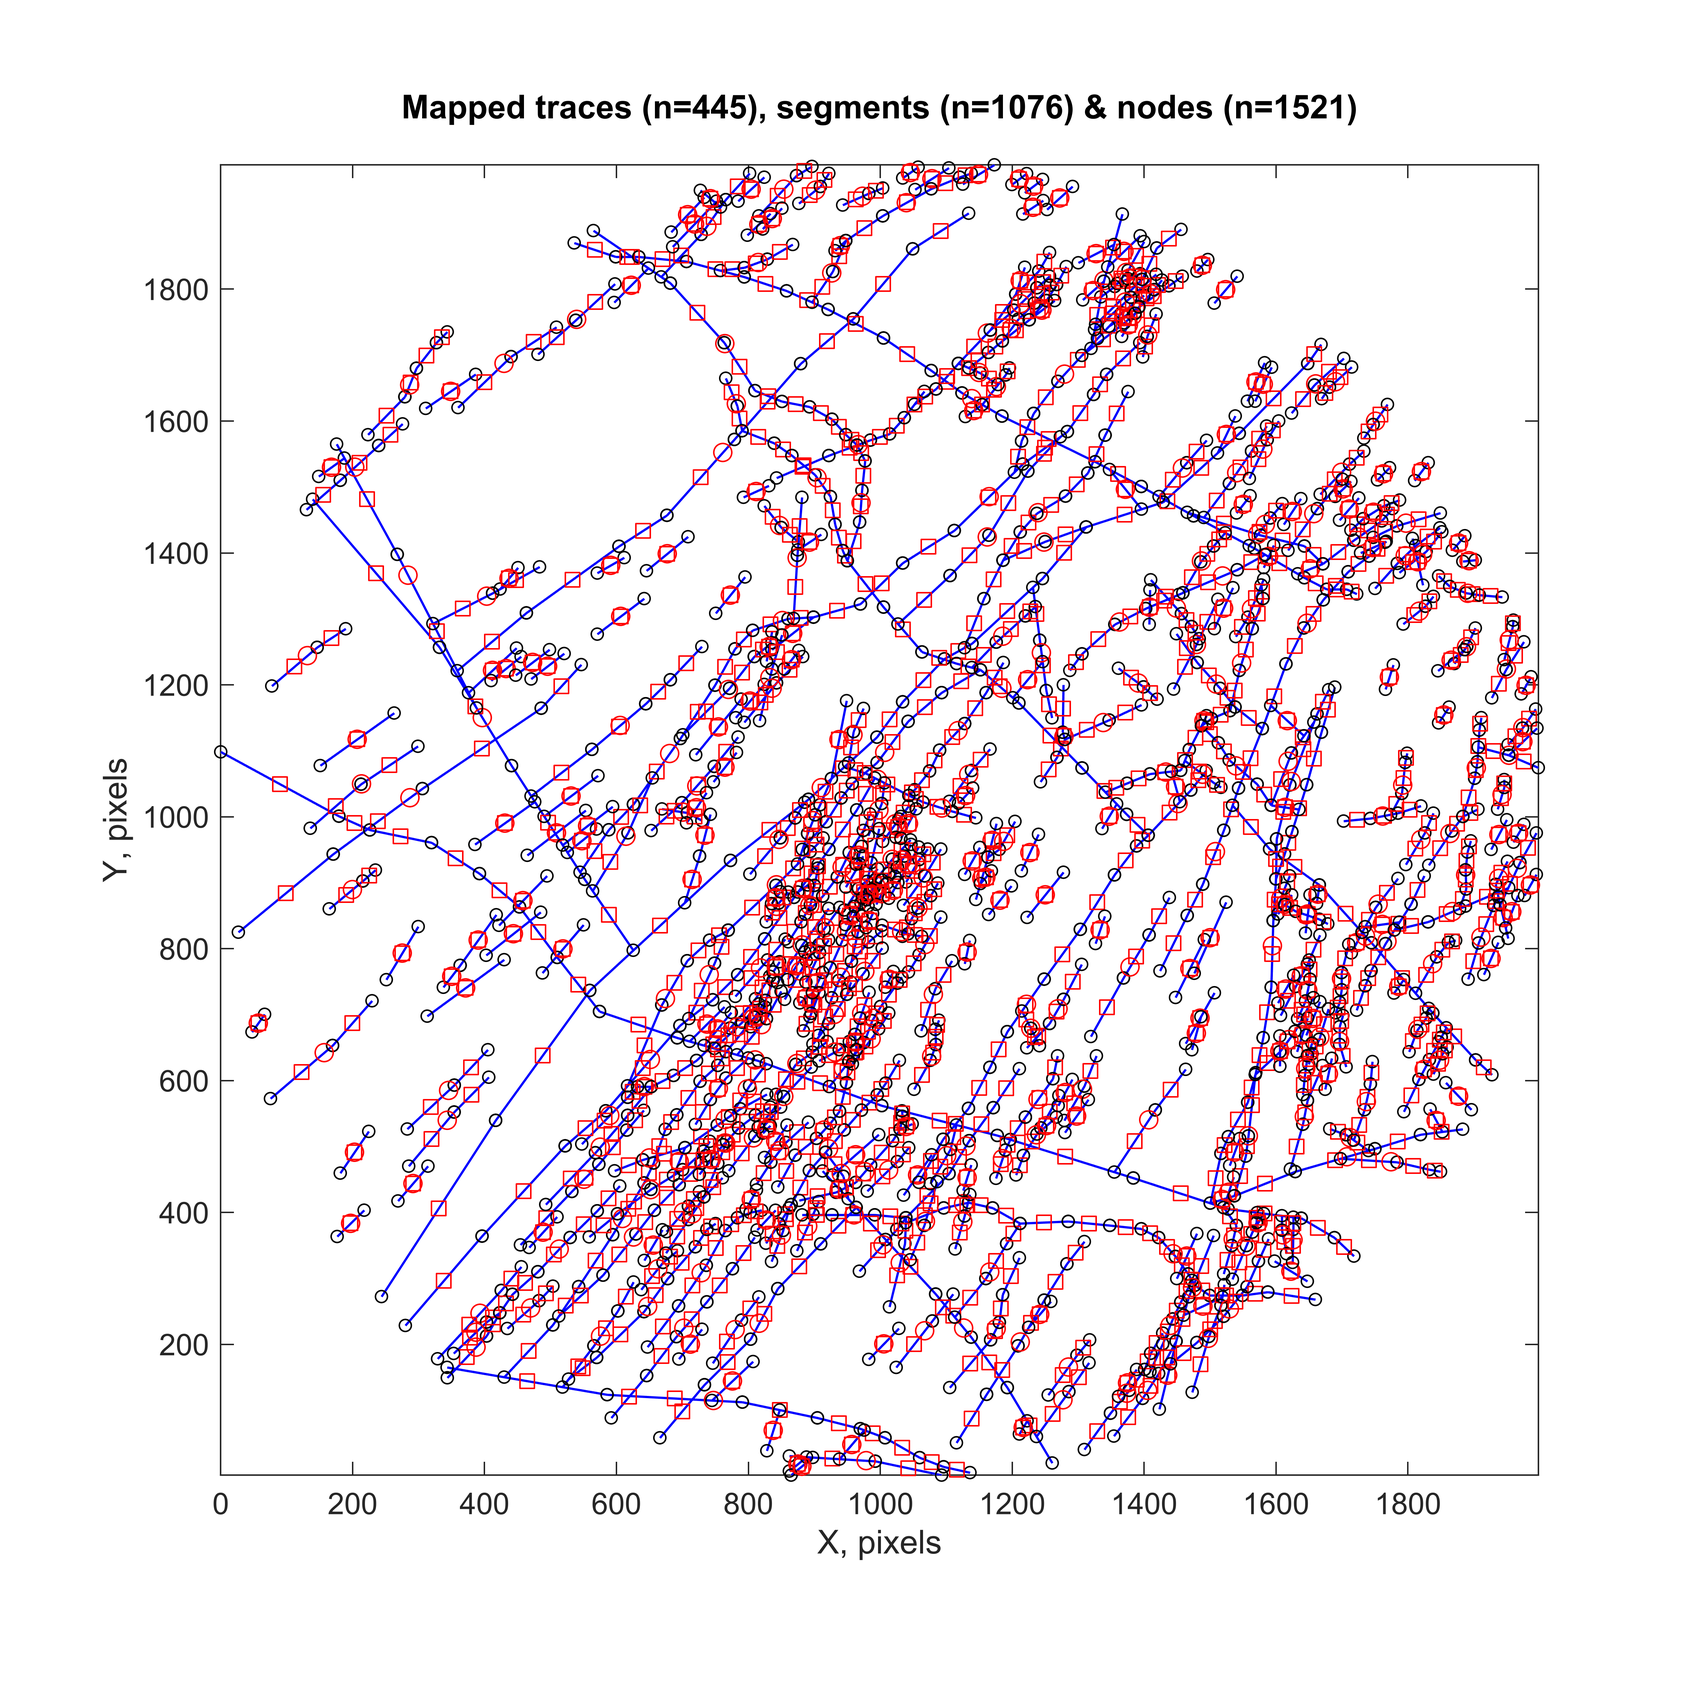
\includegraphics[width=.60\linewidth]{tracemap.png}
\vfill
{\small Implementação Python baseada no FracPaQ MATLAB 2.8.\par
Código executado localmente; não requer MATLAB.\par
Contato: \href{mailto:luismauricio@me.com}{luismauricio@me.com}.}
\end{titlepage}
\section*{Como usar este manual}
\addcontentsline{toc}{section}{Como usar este manual}
Comece pelas Seções~\ref{sec:inicio}--\ref{sec:roteiro} para preparar o ambiente, entender os dados e executar o primeiro exemplo. Depois, consulte a seção correspondente à aba desejada. Cada recurso apresenta os controles, uma interpretação do cálculo e as saídas. Os nomes dos controles permanecem em inglês para coincidir com a interface.

O exemplo principal é \code{examples/SD11A.txt}, copiado sem alterações da distribuição FracPaQ fornecida pelo mantenedor. Os resultados ilustrados usam pixels, sem calibração física. Não interprete esses pixels como metros nem os parâmetros ilustrativos de tensões e abertura como medições dessa amostra.

As figuras analíticas são resultados Python revisados; as capturas da interface mostram os widgets reais em uma janela de ilustração de 1250\,\(\times\)\,739 pixels. A janela real abre com a largura útil da tela, e aparência/tamanho podem variar com o monitor. Nas páginas seguintes, os painéis das abas foram recortados apenas para facilitar a leitura.

\begin{note}{Escopo científico}
O programa descreve traços bidimensionais. Intensidade, conectividade, tensores e permeabilidade são estimativas sob as hipóteses apresentadas; não constituem simulação completa de fluxo ou reconstrução de fraturas 3D. As correções aprovadas em relação ao legado estão resumidas na Seção~\ref{sec:limites}. A referência MATLAB é a versão 2.8; 0.9.0rc1 é a versão deste port Python.
\end{note}
\clearpage
\tableofcontents
% !TeX root = ../pyfracpaq-user-manual.tex
\major{Preparar o ambiente e iniciar}\label{sec:inicio}
Obtenha a pasta do código pelo GitHub, por clone ou download ZIP. Abra a pasta que contém \code{run_gui.py} e \code{requirements.txt}. O uso normal exige Python 3.13 e as bibliotecas; não é necessário instalar o pacote PyFracPaQ.

\subsection{Python e ambiente virtual}
No macOS, com Python 3.13 disponível, execute na raiz:
\begin{verbatim}
python3.13 -m venv .venv
.venv/bin/python -m pip install -r requirements.txt
.venv/bin/python -m pip check
.venv/bin/python run_gui.py
\end{verbatim}
Uma alternativa, na mesma pasta, é \code{.venv/bin/python -m pyfracpaq}. A instalação inicial das bibliotecas pode exigir internet. Depois, as análises funcionam localmente. Não altere silenciosamente as versões fixadas em requirements.txt.

\subsection{Miniforge e VS Code}
Com Miniforge, prepare um ambiente separado:
\begin{verbatim}
conda create -n pyfracpaq python=3.13 pip
conda activate pyfracpaq
python -m pip install -r requirements.txt
python -m pip check
python run_gui.py
\end{verbatim}
No VS Code, abra a pasta e use \control{Python: Select Interpreter}. Selecione o Python da \code{.venv} ou do ambiente Miniforge. Execute \code{run_gui.py} ou uma das configurações de Run and Debug. A extensão Python atende à seleção/execução; Python Debugger é necessária às configurações de depuração.

Foram verificados CPython 3.13.18 e Miniforge/Python 3.13.13 no macOS arm64. Windows/Linux ficam para testes posteriores do mantenedor; não se declara certificação dessas plataformas. Um ambiente chamado pyfracpaq pode já existir com outra versão: confira \code{python --version} antes de instalar.

\subsection{O que é necessário na pasta}
O programa usa \code{pyfracpaq/}, seus recursos, o launcher e as bibliotecas. \code{examples/} e este manual ajudam no uso. Testes, relatórios de auditoria e scripts internos são material de desenvolvimento do clone completo; não são necessários para executar. O ZIP de uso os exclui. Não é necessário manter a distribuição MATLAB na pasta.

\subsection{Diretório de trabalho e arquivos existentes}
A saída normal é o diretório corrente de execução. Ao iniciar pela raiz, os resultados ficam nessa raiz; para trabalhos separados, use uma cópia de trabalho ou inicie com o caminho absoluto de \code{run_gui.py} a partir da pasta de saída, usando o mesmo Python preparado. O modo por módulo, sem instalar o projeto, deve ser iniciado na raiz.

A mesma tag reutiliza os mesmos nomes e substitui arquivos anteriores. Alguns intermediários têm nomes fixos e não recebem tag. Preserve as entradas originais e separe trabalhos antes de clicar Run. A conversão SVG é uma exceção de destino: seus TXT ficam ao lado do SVG.

\major{Dados, geometria, escala e orientação}\label{sec:dados}
\subsection{Traço, segmento e nó}
Um \emph{traço} é a polilinha de uma fratura mapeada. Seus vértices são nós de entrada; dois nós consecutivos formam um segmento. Esses nós geométricos não são automaticamente os nós topológicos I/Y/X, calculados depois.

Para \(\mathbf p_i=(x_i,y_i)\),
\begin{equation}
\ell_i=\|\mathbf p_{i+1}-\mathbf p_i\|_2,
\qquad L=\sum_i\ell_i.
\end{equation}
O comprimento total \(L\) é o percurso, não a distância reta entre as pontas. O centro de um traço é interpolado a metade do percurso; o centro de um segmento é a média de suas duas pontas. Essas posições entram nos perfis e no variograma.

A área de amostragem usual é o retângulo do domínio,
\begin{equation}
A=(x_{\max}-x_{\min})(y_{\max}-y_{\min}).
\end{equation}
Não confunda essa área com a soma das áreas de blocos. Em imagens, algumas análises usam o domínio completo da imagem e os tensores usam o envelope dos nós extraídos; a área pertinente é explicitada na seção de cada família.

\subsection{Arquivo TXT de nós}
Há um traço por linha e pares X/Y separados por TAB, sem cabeçalho. Exemplo com dois traços:
\begin{verbatim}
0<TAB>0<TAB>4<TAB>0
1<TAB>2<TAB>4<TAB>2<TAB>4<TAB>6
\end{verbatim}
Substitua \code{<TAB>} por um tabulador real. O primeiro traço contém um segmento; o segundo, dois. Cada linha precisa de pelo menos dois nós distintos. Valores vazios, não finitos ou pares incompletos são recusados com localização do erro, sem leitura parcial. Duplicatas consecutivas são removidas com diagnóstico; um traço que se torna degenerado é recusado.

\subsection{Escala física}
Em \control{Scaling (pixels/metre)}, informe \(s>0\) para uma calibração conhecida. Sem escala, a unidade é pixel. O código reconstrói a geometria a partir da entrada:
\begin{equation}
 x_m=x_{px}/s,\quad y_m=y_{px}/s,\quad
 L_m=L_{px}/s,\quad A_m=A_{px}/s^2.
\end{equation}
Não basta mudar o rótulo. Uma nova escala exige nova prévia e limpa a linha de Graphs. Intensidade tem unidade de comprimento inverso, densidade de área inversa e permeabilidade de área. A abertura digitada em Fluid flow precisa estar na unidade corrente; seu número não é convertido automaticamente quando a escala muda.

\subsection{Flips, norte e ângulos}
O ângulo bruto de um segmento é medido em relação ao eixo Y, como uma direção axial, normalmente representada em \([0,180]\). Uma expressão geométrica equivalente é
\(\beta=\operatorname{atan2}(\Delta x,\Delta y)\), com a representação axial do programa. Norte, arredondamentos e flips são aplicados pelas rotinas específicas; não alteram os nós armazenados.

\control{Flip X-axis} e \control{Flip Y-axis} refletem a apresentação e influenciam as correções angulares das famílias pertinentes. \control{Rotate Y-axis from N (°)}, disponível nas abas que o utilizam, corrige o referencial angular. Perfis de ângulo em Graphs e o TXT bruto de ângulos/comprimentos não recebem a mesma transformação do EZROSE. Wavelets trabalha em seu raster e não aplica a correção de norte.

\begin{note}{Evitar duas correções da mesma geometria}
Não redesenhe os nós para compensar um flip que já será aplicado na interface. Confira a direção conhecida de uma fratura antes de interpretar rosas, tensores ou tensões. As diferenças entre os arquivos angulares são intencionais, não sinônimo de erro de unidade.
\end{note}

\subsection{SVG: conjuntos por cor}
Aceitam-se \code{line}, \code{polyline} e caminhos absolutos M/L, com stroke hexadecimal por atributo, estilo inline ou grupo. O exemplo \code{examples/colours.svg} contém duas cores. Curvas, transformações, polígonos SVG e CSS externo/classes não são convertidos silenciosamente: prepare o arquivo no editor externo.

Preview converte os nós em TXT junto ao SVG, agrupando por cor. Os nomes incluem \code{_colourHHHHHH_converted.txt}; um conjunto simples usa \code{_converted.txt}. É possível recarregar um TXT de cor para análise individual. Quando pertinente, um SVG multicolorido acrescenta a figura multicolorida; cor é procedência do conjunto, não uma classe estatística inferida.
\plotfig{tracemap_multicolour.png}{Exemplo auxiliar SVG, distinto de SD11A: preservação dos grupos de cor em mapa de traços.}{fig:svg}

\subsection{Imagens: transformada de Hough}\label{sec:hough}
Escolha JPEG/TIFF grayscale de oito bits, quadro único. RGB, alpha, imagens indexadas e maior profundidade não são convertidos automaticamente pela GUI. Use o utilitário de pré-processamento quando necessário e confira seu resultado visualmente.

O complemento identifica pixels diferentes de branco, remove pixels isolados e calcula a Hough padrão:
\begin{equation}
\rho=x\cos\theta+y\sin\theta.
\end{equation}
Uma linha de pixels acumula votos no espaço \((\theta,\rho)\). O programa usa passo angular de \(0{,}5^\circ\), passo de \(\rho\) de um pixel e coordenadas finais de imagem em base 1. Isso detecta segmentos retos: não substitui uma digitalização interpretativa de fraturas curvas.

\begin{tabularx}{\linewidth}{@{}p{.35\linewidth}X@{}}
\toprule Controle & Efeito no Preview de imagem\\\midrule
\control{Number of Hough peaks} & Limite de picos: inteiro de 100 a 5000; mais picos podem incluir ruído.\\
\control{Hough threshold} & Fração do máximo do acumulador: \(0<t\leq1\). Menor limiar inclui picos mais fracos.\\
\control{Merge gaps less than} & FillGap: distância em pixels usada para unir trechos compatíveis; maior que 1.\\
\control{Discard lengths less than} & MinLength: comprimento mínimo em pixels; maior que 1.\\\bottomrule
\end{tabularx}
Os defaults são 1000, 0.33, 5 e 3. Alterá-los exige nova prévia. A figura diagnóstica é exportada no Preview, antes do Run. Se nenhuma linha for encontrada, o diagnóstico permanece disponível, mas não há rede para analisar. O exemplo \code{examples/network.tif} é apropriado para testar esse fluxo.
\plotfig{Houghstuff.png}{Diagnóstico Hough do exemplo auxiliar de imagem. Os parâmetros são os defaults; não é uma rasterização do SD11A.}{fig:hough}

\major{Primeiro roteiro com SD11A}\label{sec:roteiro}
\subsection{Carregar e conferir a prévia}
\begin{enumerate}
\item Abra o programa e mantenha \control{Node file}.
\item Use Browse ou informe o caminho de \code{examples/SD11A.txt}.
\item Deixe a escala vazia, sem flips, e clique \control{Preview}.
\item Confira os números da tabela abaixo. As seis abas ficam disponíveis depois de uma prévia válida.
\item Troque \control{Filename tag for this run} para \code{SD11A}; escolha as saídas e clique \control{Run}.
\end{enumerate}
\begin{center}\begin{tabular}{@{}lr@{}}\toprule
Grandeza & Valor de referência\\\midrule
Traços / segmentos / nós & 445 / 1076 / 1521\\
\(x_{\min},x_{\max}\) & 0 ; 1997.7\\
\(y_{\min},y_{\max}\) & 1.8 ; 1988.5\\
Área do envelope & 3968830.59 pixels\(^{2}\)\\\bottomrule
\end{tabular}\end{center}
\begin{figure}[htbp]\centering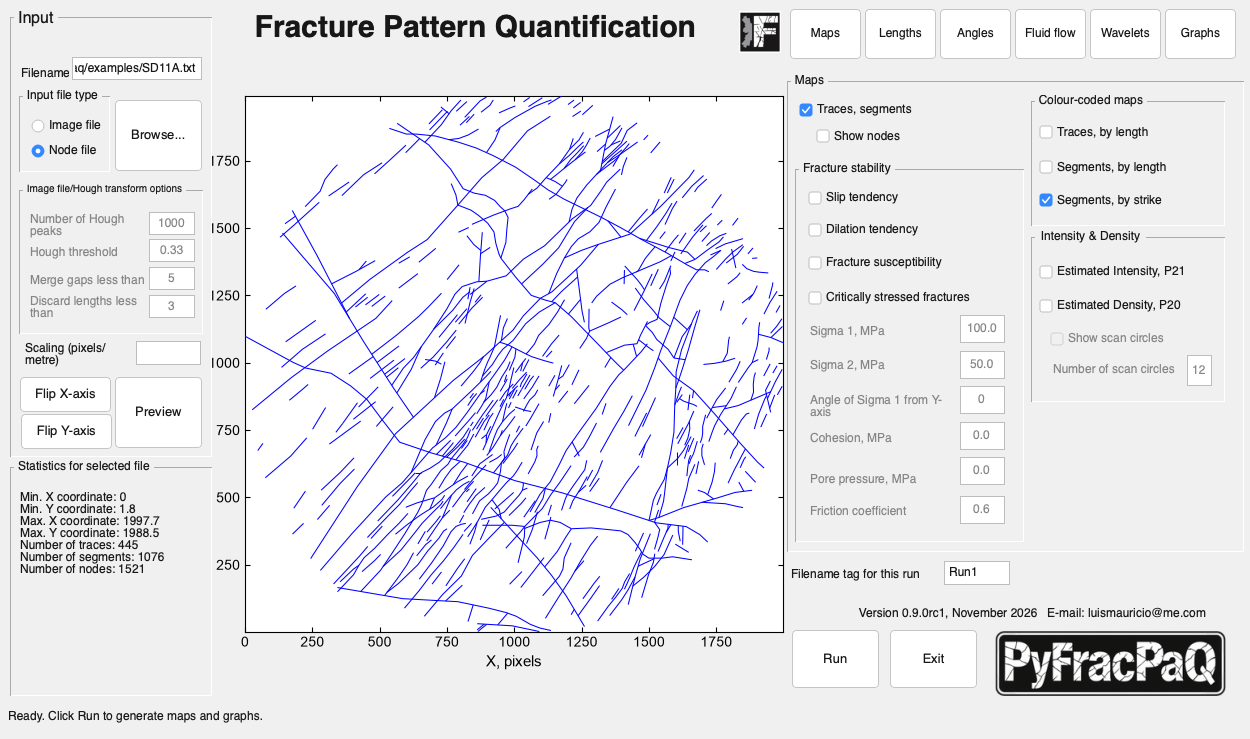
\includegraphics[width=\linewidth]{ui-preview.png}\caption{Prévia real de SD11A e estatísticas. A captura conserva a tag default Run1; use SD11A no roteiro para distinguir seus arquivos.}\label{fig:preview}\end{figure}

\Needspace{14\baselineskip}
\subsection{Parâmetros das figuras deste manual}\label{sec:parametros}
As ilustrações analíticas reutilizam uma execução revisada do SD11A com estes parâmetros, que \emph{não são todos os defaults da GUI}:
\begin{longtable}{@{}p{.43\linewidth}p{.49\linewidth}@{}}
\toprule Grupo & Configuração ilustrada\\\midrule\endhead
Entrada & Sem escala física, sem flips, norte \(0^\circ\), tag SD11A.\\
Comprimentos & 20 intervalos solicitados; censura desligada; cortes MLE Lower=0 e Upper=0.\\
Ângulos & 20 intervalos solicitados no histograma; rosa de \(10^\circ\), sem ponderação por comprimento; cor/média ativadas.\\
Maps circular & 12 círculos no lado menor; Show scan circles ativado.\\
Conectividade & 12 blocos; tolerância I\(\to\)Y de 2.0 pixels.\\
Tensões & \(\sigma_1=100\), \(\sigma_2=50\) MPa; azimute \(0^\circ\), coesão=0, pressão de poros=0, atrito=0.6. Valores ilustrativos.\\
Permeabilidade & Abertura fixa 0.001 pixel, \(\lambda=1\); exemplo sem calibração física.\\
Wavelets & Morlet, a=32, L=2, incremento \(90^\circ\). É uma grade curta de demonstração.\\
Graphs & Linha horizontal de \((0,995.15)\) a \((1997.7,995.15)\), 12 círculos.\\\bottomrule
\end{longtable}
Graphs recebe pontos por cliques, não por campos de coordenadas. A linha exata das figuras foi definida no roteiro de comparação; uma seleção manual aproximada pode mudar as interseções. MLE usa uma seed registrada na execução ilustrada; a GUI gera seeds próprias, portanto avaliações Monte Carlo podem variar.

\subsection{Estados, progresso e revisão das saídas}
Editar entrada, escala, tipo ou parâmetros Hough invalida a prévia. Run fica desabilitado enquanto não houver geometria válida ou enquanto houver operação em andamento. Apenas parâmetros necessários às análises selecionadas são validados. Uma mensagem inválida identifica o campo/aba para correção; seleções em outras abas permanecem disponíveis.

O cálculo ocorre em segundo plano; a apresentação/exportação das figuras é sequenciada na interface. Aguarde a conclusão: MLE e Wavelets podem demorar. A janela principal não possui um botão Cancel geral; Exit solicita encerramento em uma etapa segura. As figuras são janelas independentes com a barra de ferramentas Matplotlib para navegação; fechá-las não altera os dados.

% !TeX root = ../pyfracpaq-user-manual.tex
\major{Maps: geometria, amostragem e estabilidade}\label{sec:maps}
A aba reúne mapas de traços/segmentos, atributos, amostragem circular e estabilidade. Escolha somente as opções necessárias. Show nodes e Show scan circles modificam as saídas relacionadas; não são análises independentes.
\uifig{ui-maps.png}{Painel Maps. Os parâmetros de estabilidade ficam ativos quando uma opção dessa família é selecionada.}{fig:ui-maps}

\feature{MAP-01}{Traces, segments e Show nodes}
\textbf{Como usar.} Marque \control{Traces, segments}. Ative \control{Show nodes} para desenhar os vértices de entrada sobre os traços e clique Run. Uma polilinha é uma fratura mapeada; suas partes retas são segmentos, não necessariamente fraturas distintas.

\textbf{Interpretação.} Use esse mapa para identificar falhas de leitura, traços isolados, segmentação excessiva e fronteiras. A opção de nós ajuda a perceber onde um traço foi subdividido. Nós geométricos coincidentes não garantem conexão hidráulica nem classificação topológica.

\textbf{Saída.} Um mapa de traços. Para SVG com vários grupos de cor, as seleções de mapas pertinentes também acrescentam o mapa multicolorido, uma vez por Run.
\plotfig{tracemap.png}{Traços SD11A com nós geométricos, na configuração ilustrada. O domínio continua em pixels.}{fig:traces}

\feature{MAP-04}{Traces, by length}
Atribui a todos os segmentos de cada traço a cor associada ao seu comprimento total \(L\). Se uma fratura foi dividida em várias linhas no TXT, cada linha terá seu próprio comprimento; a interpretação depende da digitalização.

Marque \control{Traces, by length} e Run. Não é necessário marcar o histograma de Lengths. O comprimento usado é o percurso, inclusive em traços curvos. A escala física transforma os valores antes da análise.
\plotfig{tracelengthmap.png}{SD11A colorido pelo comprimento total do traço.}{fig:tracelength}

\feature{MAP-05}{Segments, by length}
Marque \control{Segments, by length} para colorir cada parte reta pelo seu próprio \(\ell_i\). Compare com o mapa anterior: uma fratura longa pode conter segmentos curtos devido à forma ou à resolução da digitalização.

\begin{note}{Convenção de cor dos mapas de comprimento}
O port conserva a convenção aprovada do legado: o índice da cor é linear em relação a \(L/L_{\max}\), enquanto a barra usa escala logarítmica. Portanto, a cor de uma linha não deve ser lida como uma transformação logarítmica exata do comprimento. Para valores quantitativos, use os TXT da família Lengths.
\end{note}
\plotfig{segmentlengthmap.png}{SD11A colorido por comprimento dos segmentos; note a diferença em relação ao traço inteiro.}{fig:segmentlength}

\feature{MAP-06}{Segments, by strike}
Marque \control{Segments, by strike} para mapear a orientação dos segmentos. Ajuste \control{Rotate Y-axis from N (°)} na aba pertinente e os flips conforme o referencial dos dados. A cor corresponde à orientação axial corrigida, não ao sentido de fluxo.

Segmentos paralelos com sentidos de digitalização opostos pertencem à mesma orientação axial. Arredondamento e a representação de zero como \(180^\circ\) em certas rotinas seguem a convenção da referência. Use o histograma/rosa para resumir as famílias, não apenas a impressão visual do mapa.
\plotfig{segmentstrikemap.png}{Mapa de strike do SD11A, norte zero e sem flips.}{fig:strike}

\subsection{Fundamento da amostragem circular}\label{sec:circular}
A amostragem usa janelas circulares internas ao domínio. \control{Number of scan circles} é a quantidade de círculos ao longo do lado menor, não o número total. O mínimo é 2. Para amplitude menor \(D\) e valor \(N\), o passo é \(D/(N+1)\) e \(r=0.99D/[2(N+1)]\); a quantidade no lado maior depende da razão de aspecto.

Em cada círculo, \(n\) conta encontros entre segmentos finitos e a circunferência; \(m\) conta extremidades de segmentos estritamente internas. Tangência contribui uma vez. Pontos de segmentos diferentes são contados por segmento; um vértice interno compartilhado pode contribuir duas vezes para \(m\). Uma linha totalmente interna tem \(n=0\), mas suas pontas contribuem para \(m\).
\begin{equation}
\widehat P_{21}=\frac{n}{4r},\qquad
\widehat P_{20}=\frac{m}{2\pi r^2}.
\label{eq:circle}
\end{equation}
As unidades são comprimento\(^{-1}\) e comprimento\(^{-2}\). São estimadores locais sujeitos à amostragem, não medições exatas de toda a rede dentro da janela. Círculos menores aumentam resolução espacial e variabilidade; círculos maiores suavizam a comparação.

Separadamente, o console apresenta medidas globais:
\begin{equation}
P_{21}^{\mathrm{global}}=\frac{\sum_i\ell_i}{A},\qquad
P_{20}^{\mathrm{global}}=\frac{N_{\mathrm{segmentos}}}{A}.
\end{equation}
Elas não são a média das janelas e a densidade global usa \emph{segmentos}, não traços. Para SD11A sem escala, são aproximadamente 0.01552785 pixel\(^{-1}\) e 0.000271113 pixel\(^{-2}\).

\feature{MAP-07}{Estimated Intensity, P21}
Marque a opção, informe \(N\) e, se desejar conferir a cobertura, ative \control{Show scan circles}. O Run gera o mapa de P21; Show circles acrescenta um mapa de janelas compartilhado com P20. Para o exemplo, use 12: \(r\simeq75.6474\) pixels.

Regiões quentes representam maior valor do estimador, não probabilidade de fratura. Alterar a escala ou o número de círculos muda unidades/resolução; compare mapas com parâmetros consistentes. A exportação escreve ambos os TXT de intensidade e densidade mesmo quando apenas um mapa é solicitado.
\plotfig{intensityP21.png}{P21 local do SD11A com 12 círculos no lado menor.}{fig:intensity}

\feature{MAP-08}{Estimated Density, P20 e Show scan circles}
A operação é análoga à de P21, usando a segunda expressão de~\eqref{eq:circle}. Use o mapa de círculos para verificar onde há observações e se a grade atende à escala geológica de interesse. Matrizes todas zero continuam zero; a barra recebe um intervalo gráfico representável, sem fabricar estimativas.

O port usa a contagem geométrica finita aprovada em Q-20. Uma secante cujo encontro esteja fora do segmento não é contabilizada apenas porque sua reta suporte cruza o círculo. Isso pode alterar os resultados do legado.
\plotfig{densityP20.png}{P20 local do SD11A. Unidades inversas de área e população de extremidades diferem do P21.}{fig:density}
\plotfig{scancircle.png}{Janelas efetivamente usadas nas estimativas; uma única figura é compartilhada por P21/P20.}{fig:scan}

\subsection{Fundamento dos mapas de estabilidade}\label{sec:stress}
As quatro seleções de estabilidade usam parâmetros compartilhados. Informe \(\sigma_1\geq\sigma_2>0\) em MPa, azimute de \(\sigma_1\), coesão \(C_0\geq0\), pressão de poros \(P_f\geq0\) e coeficiente de atrito \(\mu\geq0\). As tensões são compressivas positivas. Valores de abertura/permeabilidade não entram nessa família.

Para orientação corrigida \(\beta\), azimute \(\psi\) e polo relativo \(\alpha=\beta+90^\circ-\psi\),
\begin{align}
\sigma_n&=\left|\frac{\sigma_1+\sigma_2}{2}
+\frac{\sigma_1-\sigma_2}{2}\cos(2\alpha)\right|,\\
|\tau|&=\left|-\frac{\sigma_1-\sigma_2}{2}\sin(2\alpha)\right|.
\label{eq:stress}
\end{align}
Os mapas usam as orientações dos segmentos; as rosas de estabilidade avaliam os centros de classes fixas de \(10^\circ\), independentemente da largura escolhida na aba Angles. Cada opção gera mapa e rosa, e a família produz um único Mohr por Run.

\feature{MAP-11}{Slip tendency}
\begin{equation}T_s=\frac{|\tau|}{\sigma_n}.\end{equation}
É uma razão adimensional de cisalhamento/normal total. O mapa/rosa usa a normalização pelo maior \(T_s\) dos segmentos corrigidos; a cor normalizada não é o valor físico de \(T_s\). Com máximo zero, a normalização permanece zero. Comparar cores entre amostras com máximos distintos pode ser enganoso.

Marque \control{Slip tendency}, preencha as tensões e Run. Essa seleção também grava segmentdata com coordenadas e ângulos brutos; não grava \(\sigma_n\), \(\tau\) e \(T_s\) nesse TXT.
\plotfig{sliptendencymap.png}{Tendência de deslizamento SD11A sob as tensões ilustrativas, não inferidas da amostra.}{fig:slip}

\feature{MAP-12}{Dilation tendency}
\begin{equation}T_d=\frac{\sigma_1-\sigma_n}{\sigma_1-\sigma_2}.\end{equation}
Marque \control{Dilation tendency}. É um indicador de orientação favorável à dilatação dentro do estado de tensões definido. Não calcula abertura real da fratura. Exige \(\sigma_1>\sigma_2\); tensões iguais tornam o denominador indefinido e são recusadas para essa seleção.
\plotfig{dilationtendencymap.png}{Tendência de dilatação e distribuição espacial de orientações no SD11A.}{fig:dilation}

\feature{MAP-13}{Fracture susceptibility}
\begin{equation}S_f=\sigma_n-P_f-\frac{|\tau|-C_0}{\mu}.\end{equation}
Marque \control{Fracture susceptibility}; exige \(\mu>0\). \(S_f\) tem unidade MPa e representa a margem de pressão de poros no critério adotado. Valores menores indicam menor margem sob as hipóteses informadas. A escala de cor é construída com mínimo/máximo dos segmentos já corrigidos. Um campo constante recebe uma única cor/tick, sem alterar os valores físicos.
\plotfig{fracsuscepmap.png}{Suscetibilidade do SD11A, com coesão/pressão de poros zero e atrito 0.6.}{fig:suscept}

\feature{MAP-14}{Critically stressed fractures}
O critério de classificação é
\begin{equation}|\tau|\geq\mu(\sigma_n-P_f)+C_0.\label{eq:csf}\end{equation}
Marque \control{Critically stressed fractures}. A igualdade é incluída no mapa e na rosa, conforme Q-17. É uma classificação para o estado de tensões escolhido, não uma observação de fraturas ativas. Os parâmetros ilustrativos não permitem conclusão geomecânica sobre o local de coleta sem justificativa independente.
\plotfig{CSFmap.png}{Classificação CSF no SD11A. O número de fraturas críticas depende dos parâmetros, não apenas da geometria.}{fig:csf}

\subsection{Rosas de estabilidade e diagrama de Mohr}
As rosas combinam frequência de orientação e a grandeza de estabilidade avaliada no centro da classe. A linha de \(\sigma_1\) fornece referência visual. O tamanho da pétala reflete frequência, enquanto a cor codifica o indicador; não se devem confundir as duas informações.
\plotfig{sliptendencyrose.png}{Rosa de slip tendency: frequência por classe e cor normalizada pela faixa observada.}{fig:stressrose}

O círculo total tem centro \((\sigma_1+\sigma_2)/2\) e raio \((\sigma_1-\sigma_2)/2\). Com \(P_f>0\), o círculo efetivo desloca o centro por \(-P_f\). A reta de resistência é \(\tau=\mu\sigma_n'+C_0\). O port mantém o enquadramento da referência e não acrescenta pontos individuais \((\sigma_n,\tau)\) dos segmentos; sua ausência não é falha de leitura.
\plotfig{Mohrplot.png}{Mohr compartilhado pela família. Com pressão de poros zero, não há segundo círculo efetivo separado.}{fig:mohr}

% !TeX root = ../pyfracpaq-user-manual.tex
\major{Lengths: comprimentos, ajustes, blocos e variograma}\label{sec:lengths}
A família calcula comprimentos de traços e segmentos separadamente. Nos controles de classe, o valor solicitado corresponde à construção histórica de centros: por exemplo, 20 intervalos podem produzir 21 centros. Não suponha que o valor do menu seja sempre o número final de barras. A família escreve três TXT, mesmo se apenas cross-plot, blocos ou variograma estiver selecionado.
\uifig{ui-lengths.png}{Painel Lengths, com estatística descritiva, distribuições, ajustes e análises espaciais.}{fig:ui-lengths}

\subsection{Censura e estatísticas descritivas}
A opção de censura nas bordas exclui um traço inteiro se o primeiro ou o último nó tocar qualquer limite real do domínio. Todos os segmentos desse traço são excluídos pela mesma máscara, preservando a associação com seus ângulos. Não é um ajuste probabilístico para comprimentos não observados: é uma seleção geométrica de amostra.

Um vértice interno que toca a borda não equivale automaticamente a uma extremidade censurada. O domínio é definido antes da seleção. Se a censura excluir tudo, a execução é recusada antes dos arquivos dessa família, preservando os anteriores. Para reproduzir as figuras SD11A, mantenha a censura desligada.

O console informa quantidade, mínimo, máximo e média aritmética,
\(\bar L=N^{-1}\sum_i L_i\), das duas populações. Sem censura, os valores do exemplo são:
\begin{center}\begin{tabular}{@{}lrrrr@{}}\toprule
População & N & Mínimo & Máximo & Média\\\midrule
Traços &445&7.42496&2057.12077&138.48854\\
Segmentos &1076&6.32851&318.36999&57.27454\\\bottomrule
\end{tabular}\end{center}
Os valores estão em pixels. A diferença entre médias é esperada: o número de segmentos por traço varia.

\feature{LEN-02}{Histogram of lengths}
Marque \control{Histogram of lengths} e escolha a discretização. Run produz duas figuras: comprimentos de traços e de segmentos, com frequência absoluta e eixo percentual correspondente. Para uma classe com \(n_j\) observações, a frequência percentual é \(100n_j/N\).

Use esse resumo para comparar populações e identificar comprimentos dominantes, sem confundir forma do histograma com modelo estatístico. Aumentar classes reduz a quantidade por classe; extremos ficam mais instáveis. Comprimentos todos iguais são representados por uma classe, sem jitter artificial.
\plotfig{histotracelength.png}{Histograma de traços SD11A. Não é a distribuição de todos os segmentos.}{fig:lengthhist}
\plotfig{histosegmentlength.png}{Histograma de segmentos SD11A: a segmentação desloca a população para comprimentos menores.}{fig:segmenthist}

\feature{LEN-03}{Log-log lengths}
Marque \control{Log-log lengths}. São quatro gráficos: frequências por classes e frequências complementares para cada população. Os dois eixos são logarítmicos; pontos de frequência zero não são desenhados.

Conceitualmente, a frequência complementar representa observações acima de um comprimento. A implementação mantém a construção do legado:
\begin{equation}
C_j=N-\sum_{k\leq j} n_k,
\end{equation}
com \(n_k\) contados por centros de classe. Em pixels, a grade complementar usa passo unitário; em metros, 1000 intervalos (1001 centros), salvo amostra constante. Portanto, não é uma função empírica sem discretização avaliada em cada valor observado.

As figuras chamadas \emph{density distribution} mostram frequências dos histogramas em eixos log-log, não uma densidade de probabilidade normalizada por largura de classe. Uma tendência aproximadamente reta não basta para demonstrar lei de potência. Use a análise MLE e considere amostragem/censura.

A linha vertical vermelha da complementar corresponde à diagonal do domínio arredondada para cima. Ela é uma referência geométrica, não um teto imposto ao percurso de um traço curvo, que pode ultrapassá-la.
\plotfig{loglogplottracelength.png}{Complementar de comprimentos de traços. Pontos positivos são exibidos em log-log.}{fig:loglog}
\plotfig{loglogplotsegmentlengthdensity.png}{Frequências por classes dos segmentos em log-log; não são probabilidades normalizadas.}{fig:logdensity}

\feature{LEN-06}{Cross-plot lengths v angles}
Marque \control{Cross-plot lengths v angles}. Pode ser executado sozinho. Cada observação relaciona comprimento do segmento e orientação corrigida, com duplicação axial para a representação angular. A opção não relaciona comprimento total do traço com ângulo médio.

Procure se os segmentos mais longos se concentram em certas famílias; avalie o efeito da digitalização. Norte/flips pertencem à convenção angular da família. Os limites gráficos históricos podem não mostrar valores que uma correção angular legada deixa fora do intervalo; o diagnóstico e os dados preservados distinguem isso de perda na leitura.
\plotfig{crossplotsegmentlengthangle.png}{Cross-plot do SD11A: associação entre orientação e comprimento de segmentos.}{fig:cross}

\feature{LEN-07}{MLE analysis: três modelos, duas populações}\label{sec:mle}
Ative \control{Log-log lengths} e depois \control{MLE analysis}. Informe cortes percentuais Lower/Upper; para o roteiro, ambos zero. Lower remove \(\lceil Np_{\mathrm{lower}}/100\rceil\) menores valores e Upper remove \(\lceil Np_{\mathrm{upper}}/100\rceil\) maiores, após ordenação. São percentuais de observações, não comprimentos de corte na unidade do eixo.

A mesma população retida é usada na busca e no ajuste final, conforme Q-15. Para cada modelo, o programa testa limites inferiores candidatos \(x_{\min}\) e seleciona a cauda pela menor distância entre curvas complementares, com pelo menos duas observações e dois valores distintos. O menor \(x_{\min}\) vence empates. Nem todos os comprimentos precisam pertencer à cauda ajustada.

Para \(z_i\geq x_{\min}\), os estimadores adotados são
\begin{align}
\widehat\alpha&=1+\frac{n}{\sum_i\ln(z_i/x_{\min})}
&&\text{(lei de potência)},\\
\widehat\lambda&=\frac{1}{\overline{z-x_{\min}}}
&&\text{(exponencial)},\\
\widehat\mu&=\frac1n\sum_i\ln z_i,\qquad
\widehat\sigma^2=\frac1n\sum_i(\ln z_i-\widehat\mu)^2
&&\text{(lognormal)}.
\end{align}
\(\alpha\) e \(\sigma\) são adimensionais; \(\lambda\) é inverso de comprimento; \(\mu\) depende do log da unidade escolhida. O ajuste lognormal usa média/desvio dos logs da cauda, como a implementação fornecida: não é uma nova otimização de lognormal condicionalmente truncada.

As curvas usadas são
\begin{align}
S_{\mathrm{PL}}(x)&=(x/x_{\min})^{1-\alpha},\\
S_{\mathrm{Exp}}(x)&=\exp[-\lambda(x-x_{\min})],\\
S_{\mathrm{LN}}(x)&=\Phi\!\left(-\frac{\ln x-\mu}{\sigma}\right),
\end{align}
onde \(\Phi\) é a distribuição normal padrão. As figuras conservam os escalonamentos e convenções de exibição do FracPaQ. Lei de potência usa log-log, exponencial linear-log e lognormal log-linear; observe os eixos antes de comparar a curvatura.

\textbf{Saídas.} Seis figuras de ajuste: três para traços e três para segmentos. Com a seleção Log-log, há ainda os quatro gráficos dessa opção, sem recalcular a família nem duplicar os TXT. As caixas mostram parâmetros e avaliações; linhas de corte ajudam a localizar a população.
\plotfig{tracelengthsFittingPowerLaw.png}{Exemplo MLE de lei de potência para os traços SD11A. Não extrapole a reta além da cauda sem justificativa.}{fig:mlepl}
\plotfig{tracelengthsFittingExponential.png}{Exemplo exponencial para traços; a escala dos eixos difere da figura de potência.}{fig:mleexp}
\plotfig{tracelengthsFittingLogNormal.png}{Exemplo lognormal para traços. A mesma análise é feita separadamente para segmentos.}{fig:mleln}

\subsubsection{O que significam os testes e as taxas}
A distância de Kolmogorov--Smirnov compara os dois degraus empíricos:
\begin{equation}D=\sup_x|F_1(x)-F_2(x)|.\end{equation}
O procedimento conserva 2500 comparações de duas amostras por modelo, com p-valor assintótico e hipótese bilateral. A decisão usa \(p\leq\alpha_{\mathrm{sig}}\), com significância 0.1 para potência e 0.05 para exponencial/lognormal. Outra taxa contabiliza \(p>0.05\) nos três modelos. As duas quantidades não têm a mesma definição.

\begin{note}{Interpretação estatística}
As taxas não são probabilidades posteriores de um modelo ser verdadeiro. Não rejeitar não prova a distribuição, e uma reta log-log não a identifica. As seis avaliações são Monte Carlo: a GUI registra uma seed e execuções independentes podem variar. As figuras deste manual provêm de uma execução de comparação com seed registrada. Para fundamentação geral, veja Clauset et al.~\cite{clauset}; o procedimento implementado conserva particularidades do FracPaQ descritas aqui.
\end{note}

\feature{LEN-13}{Block size graphs}
Marque \control{Block size graphs}. A rede é rasterizada nas coordenadas originais, com traços de espessura definida. Componentes brancos com conectividade 8 que tocam a borda são excluídos; os restantes são interpretados como blocos fechados no raster. A seleção gera mapa de centroides, histograma de áreas e complementar log-log, além do BMP de nome fixo.

Se um componente ocupa \(n_p\) pixels e cada pixel representa \(\Delta x\Delta y\),
\begin{equation}A_b=n_p\Delta x\Delta y.\end{equation}
Centroides são calculados pelos centros dos pixels. A resolução é mantida nas coordenadas originais quando se aplica escala física; áreas mudam por \(1/s^2\) e centros por \(1/s\). A tinta do traço ocupa área: o resultado não é a área vetorial exata de um polígono. Fechamentos pequenos, lacunas e resolução podem alterar a quantidade de blocos.

O SD11A ilustrado tem 67 componentes aceitos nessa configuração. Isso não inclui a região exterior e não é uma contagem de blocos 3D. Se nenhum componente fechado existir, as figuras informam a ausência sem inventar áreas. Confira também \code{examples/rectangles.txt}: cada interior rasterizado de um quadrado de 40 por 40 mede 1444 pixels\(^{2}\), e não 1600, devido à tinta.
\plotfig{blocksizecentroidmap.png}{Centroides dos blocos identificados no raster SD11A.}{fig:blocks}
\plotfig{blocksizehisto.png}{Distribuição de áreas dos componentes aceitos. O BMP intermediário permite conferir a segmentação.}{fig:blockhist}

\feature{LEN-15}{Variogram of segment lengths}
Marque \control{Variogram of segment lengths}. As posições são os centros dos segmentos e os valores são seus comprimentos, depois da máscara comum de censura quando ativa. O semivariograma experimental por classe de distância é
\begin{equation}
\widehat\gamma(h)=\frac{1}{2N(h)}\sum_{(i,j)\in h}(\ell_i-\ell_j)^2.
\end{equation}
A distância tem unidade de comprimento e \(\gamma\), de comprimento ao quadrado. Semelhança entre segmentos próximos tende a produzir diferenças pequenas; tendências, orientação e desenho da amostragem também influenciam a curva.

A GUI usa 30 classes e distância máxima de metade da diagonal do envelope dos centros. Classes vazias ficam sem estimativa. Não há ajuste de modelo teórico, krigagem, alcance ou pepita calculados pela GUI. O comportamento histórico de pares inclui a diagonal para menos de 1000 observações e a exclui a partir de 1000; SD11A tem 1076 segmentos. Não compare populações distintas ignorando essa convenção.
\plotfig{segmentlength_variogram.png}{Semivariograma experimental do comprimento dos segmentos SD11A; nenhuma curva teórica foi ajustada.}{fig:variogram}

\major{Angles: histogramas e rosas}\label{sec:angles}
Os dados são axiais: orientações opostas representam a mesma direção de fratura. A representação circular duplica cada orientação por \(180^\circ\), depois aplica as convenções angulares pertinentes. Isso não duplica a quantidade física de segmentos.
\uifig{ui-angles.png}{Controles Angles: norte, histograma, largura angular das pétalas e opções de apresentação.}{fig:ui-angles}

\feature{ANG-01}{Histogram of angles}
Marque \control{Histogram of angles}; escolha 10, 20, 30 ou 50 intervalos solicitados. A construção histórica usa centros de 0 a \(360^\circ\), podendo produzir um centro a mais que o valor do menu. O eixo é orientação angular, não posição X/Y da rede.

A frequência conta segmentos, e a representação axial é duplicada. Se uma correção angular legada deixar valores fora de \([0,360]\), o programa diagnostica esse caso; o histograma e a rosa não o tratam como uma nova normalização silenciosa. Para comparação entre amostras, use o mesmo norte, flips e discretização.
\plotfig{histoangle.png}{Histograma angular SD11A, norte zero. Compare frequências dentro da mesma convenção axial.}{fig:anglehist}

\feature{ANG-02}{Rose diagram (equal area)}
Marque \control{Rose diagram (equal area)} e escolha pétalas de 5, 10, 20 ou \(30^\circ\). Por padrão, cada segmento contribui por contagem. \control{Length weighted?} usa os comprimentos como pesos; \control{Colour by strike?} altera a apresentação cromática e \control{Show mean vector?} acrescenta a referência de média conforme a seleção.

Se \(p_j\) é o percentual da classe, o raio é proporcional à raiz quadrada:
\begin{equation}r_j=50\sqrt{p_j}.\end{equation}
Assim, a área da pétala é proporcional ao percentual; o raio não é o próprio percentual. Na ponderação, a contribuição decorre da soma dos comprimentos da classe dividida pelo total. As classes na emenda 0/180/360 conservam os ajustes históricos do FracPaQ; não se trata de um histograma polar genérico.

As estatísticas axiais usam ângulos dobrados:
\begin{align}
C&=\frac1N\sum_i\cos(2\beta_i),\quad
S=\frac1N\sum_i\sin(2\beta_i),\quad R=\sqrt{C^2+S^2},\\
\overline\beta&=\frac12\operatorname{atan2}(S,C),\qquad
s_\beta=\sqrt{2(1-R)}.
\end{align}
A expressão de \(s_\beta\) está em radianos e é convertida para graus no programa. A média é ajustada à representação axial e as estatísticas são não ponderadas na implementação, mesmo quando a rosa é ponderada por comprimento. \(R\) próximo de zero indica média sem orientação dominante; não interprete uma linha média como direção estrutural robusta nesse caso.
\plotfig{roseangleEqArea.png}{Rosa não ponderada do SD11A, pétalas de 10 graus. O raio cresce com a raiz do percentual.}{fig:rose}

% !TeX root = ../pyfracpaq-user-manual.tex
\major{Fluid flow: topologia, crack tensors e permeabilidade}\label{sec:flow}
Os três recursos descrevem aspectos diferentes da rede. Um diagrama I/Y/X não é uma solução hidráulica, e o parâmetro \(\lambda\) da permeabilidade não é calculado automaticamente a partir dele.
\uifig{ui-fluid.png}{Controles Fluid flow: classificação topológica, tensores e abertura para a estimativa de permeabilidade.}{fig:ui-fluid}

\feature{FLO-01}{I-Y-X connectivity}
Marque \control{I-Y-X connectivity}. Informe \control{Number of blocks in maps} (inteiro \(\geq2\)) e a distância máxima de I para Y (\(\geq0\), na unidade corrente). No SD11A ilustrado, use 12 e 2.0 pixels.

A classificação segue encontros entre traços, não uma simples contagem de vértices do TXT:
\begin{itemize}
\item \textbf{I}: ponta isolada, com um ramo.
\item \textbf{Y}: junção de três ramos, incluindo T exato e proximidade de ponta real a outro segmento conforme a tolerância.
\item \textbf{X}: cruzamento de quatro ramos no modelo adotado.
\end{itemize}
A proximidade é euclidiana e inclusiva sobre segmento finito de outro traço; um undershoot pode gerar Y inferido. Um vértice interno não é tratado como ponta. T exato é Y mesmo com tolerância zero. A geometria original não é reescrita para realizar essa classificação. Sobreposições collineares e auto-interseções não equivalem automaticamente a junções entre traços.

As frações do triângulo são
\begin{equation}f_I=\frac{N_I}{N_I+N_Y+N_X},\quad f_Y=\frac{N_Y}{N_I+N_Y+N_X},\quad f_X=\frac{N_X}{N_I+N_Y+N_X}.
\end{equation}
O diagrama resume proporções, mas redes espacialmente diferentes podem ter as mesmas frações. A fundamentação topológica é discutida por Sanderson e Nixon~\cite{sanderson}; as regras concretas de proximidade do port são as descritas acima.

Run produz quatro figuras: mapa I/Y/X, calor dos nós X+Y, calor dos nós I e triângulo, além de um TXT. Para SD11A nas condições ilustradas: \(N_I=606\), \(N_Y=224\), \(N_X=90\). O TXT preserva a ordem de linhas I, X, Y; não troque as duas últimas classes ao ler o arquivo.
\plotfig{IYXnodes_traces.png}{Classificação de nós SD11A. As contagens dependem da tolerância e da digitalização.}{fig:iyxnodes}
\plotfig{IYXtriangle.png}{Triângulo topológico SD11A. Os quadrados/círculos usam formas geométricas normais.}{fig:triangle}

Os mapas de calor mostram \emph{contagens} por bloco, não densidades normalizadas por área. O número no lado maior é ajustado à razão de aspecto. A construção histórica dos bins usa o intervalo de coordenadas de cada classe não vazia, por isso os dois mapas não representam necessariamente células espaciais idênticas. Classes ausentes são tratadas sem fabricar nós.
\plotfig{XYnodes_traces_heat.png}{Contagem espacial de nós X+Y, útil para localizar concentração de junções.}{fig:xyheat}

\feature{FLO-08}{Crack tensor plot}
Marque \control{Crack tensor plot}. Para segmento \(i\), comprimento \(\ell_i\), normal unitária \(\mathbf n_i\) e área \(A\) do envelope dos nós, defina
\begin{equation}
F^{(0)}=\sum_i\frac{\ell_i^2}{A},\qquad
\mathbf F^{(m)}=\sum_i\frac{\ell_i^2}{A}\,\mathbf n_i^{\otimes m},
\quad m=2,4,8.
\end{equation}
A projeção desenhada na direção \(\mathbf v\) é
\(F_m(\mathbf v)=\sum_i(\ell_i^2/A)(\mathbf n_i\cdot\mathbf v)^m\).
São descritores angulares ponderados por comprimento ao quadrado; ordens maiores evidenciam variações direcionais de modo diferente. Não correspondem a novas dimensões espaciais do afloramento.

Run gera uma figura com ordens 0/2/4/8 e também aciona EZROSE, pois usa a família angular. O envelope precisa ter área positiva, inclusive para redes extraídas de imagem; uma linha única não permite esse cálculo. Polos usam a convenção de norte, arredondamento e flips própria da referência.
\plotfig{cracktensor.png}{Projeções dos crack tensors SD11A. A curva de ordem zero fornece a referência isotrópica do peso.}{fig:crack}

\feature{FLO-09}{Permeability plot (polar)}
Marque \control{Permeability plot (polar)}. Escolha abertura fixa \(t\geq0\) ou escalada \(t_i=a\ell_i^b\), com fator \(0\leq a\leq0.1\), expoente \(0.5\leq b\leq1\), e \(0\leq\lambda\leq1\). Apenas os parâmetros do modo ativo são usados.

O modelo de placas paralelas adotado calcula
\begin{align}
\mathbf P&=\sum_i\frac{t_i^3\ell_i}{A}\,\mathbf n_i\otimes\mathbf n_i,\\
\mathbf K&=\frac{\lambda}{12}\left[\operatorname{tr}(\mathbf P)\mathbf I-\mathbf P\right],\qquad
k(\mathbf v)=\mathbf v^{\!T}\mathbf K\mathbf v.
\end{align}
A área é o envelope dos nós, não automaticamente a área inteira da imagem. A curva polar mostra a projeção direcional; os autovalores fornecem máximos/mínimos principais. \(\mathbf K\) tem unidade de área. Sem calibração física, o resultado é pixel\(^{2}\) e não uma permeabilidade física em m\(^{2}\).

Dobrar a abertura multiplica \(\mathbf K\) por oito; \(\lambda\) atua linearmente. Abertura zero ou \(\lambda=0\) gera tensor zero. \(\lambda\) é uma escolha do usuário, independente da contagem I/Y/X. A abertura é digitada na unidade corrente; mudar escala não converte automaticamente esse número. Para abertura escalada, a unidade de \(a\) depende de \(b\).

No exemplo sem escala, com abertura fixa 0.001 pixel e \(\lambda=1\), os autovalores são aproximadamente \(2.8756\times10^{-13}\) e \(1.00643\times10^{-12}\) pixel\(^{2}\). São ilustração numérica, não estimativa física do material. Essa opção gera PNG e mensagens no console, sem um novo TXT próprio.
\plotfig{permeability_polar.png}{Projeção polar de permeabilidade do SD11A sob abertura/\(\lambda\) ilustrativos.}{fig:permeability}

\major{Wavelets 2D: escala, orientação e anisotropia}\label{sec:wavelets}
\feature{WAV-01}{Run wavelet analysis}
A análise busca estruturas orientadas em diferentes escalas de um raster da rede. Marque \control{Run wavelet analysis}, escolha Morlet ou Mexican Hat e informe listas de a, L e um incremento angular.
\uifig{ui-wavelets.png}{Painel Wavelets. As listas são números separados por espaços, não expressões MATLAB.}{fig:ui-wavelets}

\subsubsection{Parâmetros e roteiro inicial}
Use \(a=32\), \(L=2\) e incremento \(90^\circ\) para acompanhar a figura deste manual. É uma demonstração curta, não uma recomendação de resolução para pesquisa. Uma grade mais fina pode usar a=16 32, L=2 4 e incremento 30, com custo maior.

As listas a/L exigem inteiros positivos, separados por espaços; escreva \code{8 16 32}, não \code{8:8:32}. O incremento deve ser inteiro positivo divisor de \(180^\circ\), por exemplo 10, 20, 30, 45, 60 ou 90. O cálculo usa a razão anisotrópica \(r=1/L\); L=1 é isotrópico, podendo produzir orientação fisicamente indeterminada em empates.

\subsubsection{Raster e núcleos}
O raster mantém o contrato de 27 polegadas a 72 dpi: 1944\(\times\)1944 pixels, com margens e espessuras definidas. Traços de comprimento \(\geq45\%\) do maior usam 4 pontos; os demais, 1. Branco vira fundo zero na normalização. Escala física e norte não são introduzidos nas coordenadas desse raster.

Para coordenadas centradas, rotacionadas e divididas por a, \((\xi,\eta)\), e \(q=(r\xi)^2+\eta^2\), os núcleos implementados têm as formas
\begin{align}
\psi_M&=\frac{\sqrt r}{a}\exp(-2\pi\mathrm i\eta)\exp(-q/2),\\
\psi_H&=\frac{2-q}{a}\exp(-q/2).
\end{align}
A resposta é a convolução discreta da imagem sem sua média com a parte real do núcleo, calculada por FFT e recortada às dimensões originais. A resposta própria do núcleo conserva o termo complexo no caso Morlet; não é substituída por módulo ao quadrado.

A normalização usada para a seleção é
\begin{equation}
WC(a,\theta,L)=\frac{2.5\,|W|}{a\,\max|W_{\mathrm{self}}|}.
\end{equation}
Para cada posição e a, guarda-se o maior WC entre as orientações e fatores. Empates numéricos de orientação usam a primeira escolha estável, conforme Q-12. A energia registrada é a soma dos quadrados da resposta. Isso descreve a implementação do port, não uma promessa de equivalência entre todas as definições de CWT da literatura.

\subsubsection{Ler os quatro painéis e arquivos}
Cada a gera um painel 2\(\times\)2: raster de entrada, mapa WC, rosa das orientações selecionadas e histograma de \(\log_{10}\) da frequência. A máscara é fixa e estrita:
\begin{equation}WC>0.5\,\max(WC).
\end{equation}
Não há controle deslizante para esse limiar. A orientação ótima do raster é convertida para a representação axial da rosa; norte não entra, e flips seguem o contrato da família.

Cada a grava também o TXT de theta. O raster intermediário tem nome fixo sem tag. O custo cresce aproximadamente com o produto entre quantidades de a, L e orientações, além do tamanho da FFT. O programa estima memória e limita essa família a 2 GiB de trabalho; diminuir a grade pode ser necessário. Não interprete o tamanho do arquivo de entrada TXT como previsão do custo da Wavelet.
\plotfig{wavelet_a32.png}{SD11A, Morlet, a=32, L=2 e passo angular de 90 graus. A amostragem curta é ilustrativa; a barra WC não é probabilidade.}{fig:wavelet}

\major{Graphs: perfis ALONG e FROM}\label{sec:graphs}
Selecione primeiro uma linha na prévia. Clique \control{Select end points} e depois dois pontos distintos dentro do mapa, na ordem desejada. Escape ou botão direito cancelam a tentativa, preservando a última linha completa. Um segundo ponto igual ao primeiro precisa ser escolhido novamente. Cliques fora dos eixos são ignorados; Run fica desabilitado durante uma seleção incompleta.
\uifig{ui-graphs.png}{Graphs combina seleção de linha e perfis. P21/P20 compartilham os círculos dessa linha.}{fig:ui-graphs}

Entrada, escala, tipo, parâmetros Hough ou nova prévia limpam a linha; flips e norte a preservam. A linha das figuras deste capítulo vai de \((0,995.15)\) a \((1997.7,995.15)\); na GUI, a escolha é por cliques, de modo que pequenas diferenças são esperadas.

\subsection{Definições geométricas}
Para extremos \(\mathbf p_1\), \(\mathbf p_2\), vetor \(\mathbf d=(d_x,d_y)=\mathbf p_2-\mathbf p_1\) e \(D=\|\mathbf d\|\), ALONG usa o segmento finito e a distância da interseção ao ponto 1. FROM usa a reta infinita e a distância assinada de um ponto \((x,y)\):
\begin{equation}
d_\perp=\frac{d_y(x-x_1)-d_x(y-y_1)}{D}.
\end{equation}
Para linha horizontal da esquerda para a direita, pontos acima têm sinal negativo. Inverter a linha troca o sinal de FROM e a origem de ALONG. Norte e flips não corrigem os ângulos brutos desses perfis; os flips afetam seu mapa auxiliar.

ALONG conserva um registro por segmento que intersecta a linha. Um traço sinuoso pode aparecer várias vezes; um vértice compartilhado pode gerar duas observações. Contatos collineares são excluídos. Não há ordenação/deduplicação automática. Sem encontros, os perfis ALONG informam ausência de dados, sem bloquear os demais.

\feature{GRA-03}{ALONG: Trace length}
Marque a opção após escolher a linha. Cada encontro recebe, no eixo Y, o comprimento total do traço correspondente; o eixo X mede distância ao ponto 1. Um mesmo valor pode se repetir por múltiplas interseções do mesmo traço. Isso não significa duplicação do TXT de entrada.
\plotfig{tracelengthalonggraph.png}{Comprimento dos traços que intersectam a linha SD11A, ao longo do perfil.}{fig:tracealong}

\feature{GRA-04}{ALONG: Segment length}
Usa as mesmas interseções, mas desenha o comprimento do segmento encontrado, não do traço inteiro. Compare com o perfil anterior para perceber onde traços extensos foram subdivididos.
\plotfig{segmentlengthalonggraph.png}{Comprimento dos segmentos intersectados pela linha de perfil.}{fig:segmentalong}

\feature{GRA-05}{ALONG: Segment angle}
Desenha o ângulo bruto do segmento em cada interseção. Agrupamentos podem apontar mudanças de família ao longo da linha; não são uma rosa local nem ângulos médios por janela.
\plotfig{segmentanglealonggraph.png}{Ângulos brutos ao longo da linha SD11A.}{fig:anglealong}

\feature{GRA-06}{ALONG: Estimated intensity, P21}
Escolha \control{Number of scan circles} inteiro \(\geq2\). Nesta família, \(r=D/(2N)\), centros estão nas frações \((k+0.5)/N\) da linha e as abscissas vão de r a \(D-r\). Essa grade difere da grade retangular de Maps. O estimador é \(n/(4r)\) com a contagem finita já descrita.

Selecionar P21 ou P20 produz, em conjunto, mapa de círculos e ambos os perfis, uma vez por Run. Use o mapa para conferir alcance e cobertura. O mapa identifica ponto 1/ponto 2 e conserva seus marcadores de cor correspondentes.
\plotfig{graphtracemap.png}{Linha e círculos do perfil SD11A; o raio depende do comprimento da linha e de N.}{fig:graphmap}
\plotfig{intensityalonggraph.png}{Intensidade estimada ao longo do perfil, 12 círculos.}{fig:graphintensity}

\feature{GRA-07}{ALONG: Estimated density, P20}
Usa os mesmos círculos e \(m/(2\pi r^2)\). O quadrado do raio é uma correção aprovada em Q-20; não se preservou o denominador linear em r da rotina Graphs legada. A unidade é inversa de área, consistente com Maps. P21 e P20 não são a mesma informação com escala diferente: contam eventos distintos.
\plotfig{densityalonggraph.png}{Densidade estimada no mesmo perfil, com a normalização de área aprovada.}{fig:graphdensity}

\feature{GRA-10}{FROM: Trace length}
Cada traço contribui com seu centro a metade do percurso e comprimento total. A abscissa é a distância assinada desse centro à reta infinita; não exige interseção com o segmento de perfil. Não é distância da ponta mais próxima nem média de distâncias dos nós.
\plotfig{tracelengthfromgraph.png}{Comprimentos de traços em função da distância assinada de seus centros.}{fig:tracefrom}

\feature{GRA-11}{FROM: Segment length}
Cada segmento contribui com seu centro geométrico e seu comprimento. O mesmo traço pode aparecer em diversas posições por ter vários segmentos. A reta infinita permite estudar uma faixa lateral, mas não impõe uma janela de largura finita.
\plotfig{segmentlengthfromgraph.png}{Comprimentos dos segmentos em função de sua distância à reta de referência.}{fig:segmentfrom}

\feature{GRA-12}{FROM: Segment angle}
Usa os centros dos segmentos e seus ângulos brutos. Observe o sinal de distância ao comparar os dois lados da linha; inverter a linha inverte esse sinal. Graphs gera PNG, sem TXT próprio para os perfis.
\plotfig{segmentanglefromgraph.png}{Orientações de segmentos nos dois lados da linha SD11A.}{fig:anglefrom}

% !TeX root = ../pyfracpaq-user-manual.tex
\major{Ferramentas complementares}\label{sec:aux}
Use o mesmo Python preparado, na raiz do código. Com Miniforge ativado, substitua \code{.venv/bin/python} por \code{python}. Caminhos com espaços devem ficar entre aspas.

\subsection{Pré-processar fotografias para Hough}
\begin{verbatim}
.venv/bin/python -m pyfracpaq.tools preprocess foto.jpg \
  preparada.tif --panel etapas.png
\end{verbatim}
O comando aceita RGB/grayscale de oito bits e exige caminhos distintos para entrada, TIFF e painel PNG. O TIFF é grayscale binário 0/255. A conversão de cinza aproxima \(0.298936R+0.587043G+0.114021B\), com arredondamento. A mediana usa janela de 20\(\times\)20; a diferença saturada é
\begin{equation}D=\max\{\operatorname{mediana}(I)-I,0\}.\end{equation}
Seguem Sobel, fechamento morfológico e afinamento/inversão. A mediana estima o fundo; a diferença destaca estruturas escuras; Sobel responde a gradientes; fechamento/afinamento modificam conectividade e espessura. Isso pode unir ou perder traços: confira o painel antes de importar. Não há segmentação por IA.
\plotfig{preprocess.png}{Pré-processamento de uma fotografia de referência, distinta de SD11A e do exemplo Hough.}{fig:preprocess}

\subsection{Converter objetos Move em nós}
\begin{verbatim}
.venv/bin/python -m pyfracpaq.tools move \
  examples/move_objects.dat nos.txt \
  --x-column 1 --y-column 3 --skip-header 1
\end{verbatim}
As colunas começam em 1; os defaults são X=1, Y=3 e zero linhas de cabeçalho. O exemplo requer uma linha de cabeçalho. Linhas vazias separam os objetos; o último é preservado mesmo sem linha vazia final. O TXT usa quatro casas e TAB. Confira o resultado em Preview; erro de conversão não substitui o arquivo anterior.

\subsection{Diálogo Wavelets sobre raster existente}
\begin{verbatim}
.venv/bin/python -m pyfracpaq.tools wavelet-dialog \
  FracPaQ2D_wavelet_traces.png \
  --output-directory . --tag Run1
\end{verbatim}
O diálogo aceita raster L/RGB de oito bits e reutiliza os kernels/parâmetros da Seção~\ref{sec:wavelets}. Run congela a configuração e processa seu próprio trabalho; Cancel solicita interrupção em uma etapa segura ou fecha apenas o diálogo. A prévia principal não é substituída. PNGs recebem a tag da ferramenta; TXT theta mantém o nome auxiliar \emph{sem tag}. Alterar somente --tag não separa esses TXT.

\subsection{APIs e legado}
Variograma avançado, tensor 16, rosas lineares/históricas, probePlane, leitor textual genérico e paletas também existem por APIs Python. Não são controles adicionais da GUI 2.8. Experimentos incompletos/interfaces antigas são referência, sem novos botões. Seus contratos estão na documentação de desenvolvimento; o uso comum das abas não depende deles.

\major{Arquivos de saída e organização}\label{sec:exports}
\subsection{Figuras, tags e quantidades}
Os PNGs analíticos usam 20\(\times\)20 cm a 600 dpi, ou 4724\(\times\)4724 pixels no backend verificado. O tamanho na tela não altera essa resolução. Barras horizontais acompanham a largura do plot e verticais sua altura, mantendo distância fixa aos rótulos.

A maioria dos nomes segue \code{FracPaQ2D_nome_SD11A.png}. Graphs usa \code{guiFracPaQ2D_}; Wavelets usa, por exemplo, \code{FracPaQ2Dwavelet_a32_SD11A.png}. O underscore antes da tag permanece com tag vazia. Espaços/acentos são aceitos; separadores de caminho/caracteres reservados são recusados. A tag não escolhe pasta.
\begin{longtable}{@{}p{.29\linewidth}p{.63\linewidth}@{}}
\toprule Seleção & PNGs por Run\\\midrule\endhead
Traços/comprimento/strike & Um por seleção; SVG pode acrescentar mapa multicolorido.\\
P21/P20 em Maps & Um por mapa; Show circles acrescenta mapa compartilhado.\\
Estabilidade & Mapa e rosa por opção; um Mohr para a família.\\
Histogramas Lengths & Dois, traços e segmentos.\\
Log-log lengths & Quatro, frequências por classe/complementares das duas populações.\\
MLE & Seis adicionais, três modelos por população.\\
Cross-plot/variograma & Um por seleção.\\
Blocos & Três: centroides, histograma e complementar.\\
Histograma angular/rosa & Um por seleção.\\
I-Y-X & Quatro: nós, calor X+Y, calor I e triângulo.\\
Tensores/permeabilidade & Um por seleção.\\
Wavelets & Um painel por a, além do raster fixo.\\
Graphs & Um por perfil de atributo; P21/P20 compartilham mapa e os dois perfis circulares.\\
Preview de imagem & Diagnóstico Hough antes de Run.\\\bottomrule
\end{longtable}
O Run padrão gera cinco PNGs e quatro TXT. Uma checkbox não corresponde necessariamente a um único arquivo.

\subsection{TXT e intermediários}\label{sec:txt}
Os nomes abaixo usam tag SD11A e a=32. Os TXT não têm cabeçalho, salvo letras de classe na conectividade.
\begin{longtable}{@{}p{.54\linewidth}p{.38\linewidth}@{}}
\toprule Arquivo & Conteúdo\\\midrule\endhead
\code{FracPaQ2Dsegmentlengths_SD11A.txt} & Segmentos ordenados; duas casas.\\
\code{FracPaQ2Dtracelengths_SD11A.txt} & Traços ordenados; duas casas.\\
\code{FracPaQ2Dsegmentangleslengths_SD11A.txt} & Ângulo bruto/comprimento, ordem original alinhada; duas casas.\\
\code{FracPaQ2DEZROSE_SD11A.txt} & Ângulos corrigidos, axiais duplicados e ordenados; duas casas.\\
\code{FracPaQ2Dintensity_SD11A.txt} & X/Y/P21; centros com uma casa, estimativa com oito.\\
\code{FracPaQ2Ddensity_SD11A.txt} & X/Y/P20, X por fora/Y por dentro.\\
\code{FracPaQ2Dconnectivity_SD11A.txt} & Linhas I, X e Y e suas contagens.\\
\code{FracPaQ2Dsegmentdata_SD11A.txt} & Sequência base 1, X1/Y1/X2/Y2 com quatro casas, ângulo bruto com uma.\\
\code{FracPaQ2Dwavelet_theta_a32_SD11A.txt} & Orientações da aba principal, uma por linha.\\
\code{nome_converted.txt} /\newline\code{nome_colourHHHHHH_converted.txt} & Nós do SVG junto à origem; por cor quando necessário.\\
\code{FracPaQ2D_blocksize.bmp} & Raster de blocos, fixo sem tag.\\
\code{FracPaQ2D_wavelet_traces.png} & Raster Wavelets 72 dpi, fixo sem tag.\\
\code{FracPaQ2Dwavelet_theta_a32.txt} & Theta do diálogo auxiliar, sem tag.\\\bottomrule
\end{longtable}
Lengths grava seus três TXT quando a família é selecionada. Angles/crack tensor aciona EZROSE. P21 ou P20 em Maps escreve ambos os TXT circulares. Somente Slip tendency grava segmentdata. Graphs não tem TXT próprio. Preprocess grava nos caminhos fornecidos; seu painel tem resolução distinta dos PNGs analíticos.

A precisão histórica arredonda valores textuais: centros diferentes podem aparecer iguais em unidades pequenas. Arrays internos mantêm precisão. Não reimporte tabelas estatísticas como TXT de nós.

\subsection{Substituição e execução parcial}
Cada arquivo é preparado em temporário próprio e substituído atomicamente. Não há transação única para o Run. Uma falha/interrupção pode deixar arquivos de execuções diferentes; confira mensagens e pasta. O erro não desfaz automaticamente todos os arquivos, e não há limpeza genérica de arquivos alheios.

\major{Interpretação e solução de problemas}\label{sec:limites}
\subsection{Sequência para uma análise responsável}
\begin{enumerate}
\item Confira geometria/estatísticas e decida calibração antes de interpretar unidades.
\item Compare mapas com histogramas/rosa; avalie segmentação e referencial angular.
\item Experimente resoluções P21/P20 justificadas e registre N/raio.
\item Justifique a tolerância topológica pela digitalização, não pela aparência desejada do triângulo.
\item Decida censura antes dos ajustes de cauda; registre cortes e parâmetros.
\item Oriente perfis por uma pergunta geológica; declare pontos, direção e unidade.
\item Só interprete fisicamente permeabilidade/estabilidade com abertura e tensões independentes justificadas.
\item Em Wavelets, explicite raster, a, L e incremento angular.
\end{enumerate}

\subsection{Diferenças aprovadas}
Q-05 usa censura por traço; Q-11, proximidade de pontas reais. Q-12 define o raster, as dimensões e os desempates de Wavelets. Q-14 exclui o exterior e calibra blocos. Q-15 corrige cortes e busca de caudas. Q-17 corrige normalização, cores e igualdade CSF. Q-20 usa contagem finita e P20 por área. São padrões ativos e podem diferir do legado.

Foram preservadas as convenções de ângulo bruto/corrigido e de índices lineares com barra logarítmica nos mapas de comprimento. Foram aceitas diferenças visuais em cinco títulos e duas vistas Hough, sem autorizar mudar acumuladores/picos/endpoints. Marcadores usam quadrados/círculos normais. Isso não declara identidade geral de pixels, equivalência com resultados corrigidos do legado ou adequação a qualquer amostra. Os detalhes das auditorias são opcionais no clone completo.

\Needspace{27\baselineskip}
\subsection{Diagnósticos frequentes}
\begin{longtable}{@{}p{.34\linewidth}p{.58\linewidth}@{}}
\toprule Situação & Verificação\\\midrule\endhead
Run desabilitado & Atualize a prévia; aguarde a operação; termine/cancele a linha de perfil.\\
TXT recusado & TAB, pares completos, sem cabeçalho, valores finitos, dois nós distintos por traço.\\
SVG recusado & Prepare curvas, transformações e CSS no editor; não apenas troque a extensão.\\
Imagem recusada & Grayscale oito bits, JPEG/TIFF, quadro único; RGB/alpha exige preparo.\\
Hough sem linhas & Confira branco/fundo, limiar, FillGap e MinLength no diagnóstico.\\
Tensor/Maps circular falha & Verifique área bidimensional positiva.\\
MLE sem amostra & Reveja censura/cortes; a cauda precisa de dois valores distintos.\\
Blocos ausentes & Confira fechamento, tinta e resolução no BMP.\\
ALONG vazio & A linha finita precisa encontrar segmentos não collineares; FROM é diferente.\\
Wavelets demorada & Reduza a, L e orientações e respeite a memória.\\
Permeabilidade em pixel\(^{2}\) & Falta escala física; não renomeie o eixo para metros.\\
ModuleNotFoundError & Confira interpretador, pasta raiz e requirements.txt com o mesmo Python.\\\bottomrule
\end{longtable}

\subsection{Registro mínimo para reprodução}
Guarde entrada/checksum, versão, escala/unidade, norte/flips, seleções, classes, censura/cortes, tolerância, parâmetros físicos, pontos do perfil, grade Wavelets, tag e pasta. Para Monte Carlo, guarde a seed do console. A GUI não salva uma sessão geral; um PNG não registra toda a configuração.

SHA-256 do SD11A incluído:\par
{\small\ttfamily 96bafa56537444279a748c3f4b7a4300f7e7\allowbreak 3341a04d2ba4ff8cf1299ad74688.}

\major{Mapa de recursos e referências}
\subsection{Localizar cada análise}
\begin{longtable}{@{}p{.23\linewidth}p{.69\linewidth}@{}}
\toprule Aba & Recursos e páginas\\\midrule\endhead
Maps & Traços (\pageref{feat:MAP-01}); comprimentos (\pageref{feat:MAP-04}/\pageref{feat:MAP-05}); strike (\pageref{feat:MAP-06}); P21/P20 (\pageref{feat:MAP-07}/\pageref{feat:MAP-08}); estabilidade (\pageref{feat:MAP-11}--\pageref{feat:MAP-14}).\\
Lengths & Histogramas (\pageref{feat:LEN-02}); log-log (\pageref{feat:LEN-03}); cross-plot (\pageref{feat:LEN-06}); MLE (\pageref{feat:LEN-07}); blocos (\pageref{feat:LEN-13}); variograma (\pageref{feat:LEN-15}).\\
Angles & Histograma (\pageref{feat:ANG-01}) e rosa (\pageref{feat:ANG-02}).\\
Fluid flow & I/Y/X (\pageref{feat:FLO-01}); tensores (\pageref{feat:FLO-08}); permeabilidade (\pageref{feat:FLO-09}).\\
Wavelets & Kernel e seleção (\pageref{feat:WAV-01}).\\
Graphs & ALONG (\pageref{feat:GRA-03}--\pageref{feat:GRA-07}); FROM (\pageref{feat:GRA-10}--\pageref{feat:GRA-12}).\\
Complementos & Ferramentas (\pageref{sec:aux}); arquivos (\pageref{sec:exports}).\\\bottomrule
\end{longtable}

\subsection{Procedência e créditos}
As fórmulas descrevem a implementação Python 0.9.0rc1 e decisões aprovadas, conferidas em seus módulos de geometria/análise/exportação. Não se atribuem ao MATLAB resultados corrigidos do port. As origens/checksums das ilustrações estão em \code{figure-provenance.json}; exemplos auxiliares são identificados nas legendas.

SD11A foi copiado sem alterações da distribuição FracPaQ MATLAB 2.8 fornecida, com atribuição MIT. Exemplos sintéticos são do projeto. Considere a teoria e referências originais ao publicar resultados~\cite{healy}. Preserve David Healy, colaboradores e bibliotecas nos créditos LICENSE/THIRD\_PARTY\_NOTICES. Marcas e nomes identificam referências, sem implicar endosso.

\begin{thebibliography}{9}
\bibitem{healy} Healy, D. et al. (2017). \emph{FracPaQ: A MATLAB toolbox for the quantification of fracture patterns}. Journal of Structural Geology, 95, 1--16. \href{https://doi.org/10.1016/j.jsg.2016.12.003}{doi:10.1016/j.jsg.2016.12.003}.
\bibitem{clauset} Clauset, A.; Shalizi, C. R.; Newman, M. E. J. (2009). \emph{Power-Law Distributions in Empirical Data}. SIAM Review, 51(4), 661--703. \href{https://doi.org/10.1137/070710111}{doi:10.1137/070710111}.
\bibitem{sanderson} Sanderson, D. J.; Nixon, C. W. (2015). \emph{The use of topology in fracture network characterization}. Journal of Structural Geology, 72, 55--66. \url{https://www.sciencedirect.com/science/article/abs/pii/S0191814115000152}.
\end{thebibliography}

\end{document}
